\chapter{The Skein Algebra of the Torus} \label{chap:torus}

This chapter is dedicated to the study of the Dubrovnik skein algebra of a torus $\cd(T^2)$, the main result being a simple presentation for the algebra, stated in Theorem \ref{thm:toruspresentation}. The generators $\widetilde{P}_\xx$ are embeddings of certain special elements $\widetilde{P}_k \in \cd(A)$, which we define in Section \ref{sec:powersumelements}. The $\widetilde{P}_k$ generalize both the power sum elements $P_k \in \ch(A)$ and the Chebyshev polynomials $T_k \in \ck(A)$ which are both used widely in the context of their respective skein theories due to the simple relations they satisfy. In particular, we give a simple formula in Theorem \ref{thm:powersumcommutator} which explains how to move any embedding of $\widetilde{P}_k$ past a single strand in any skein module, which gives us a family of relations between the $\widetilde{P}_\xx$. In Section \ref{sec:presentation}, we show how this and another family of relations imply the relations given in the stated presentation. 

The definition of the $\widetilde{P}_k$ make it clear why these elements generalize their HOMFLYPT counterparts, but the same isn't immediately clear for the Kauffman bracket case for the $T_k$. In Section \ref{sec:compatibility} we justify this claim by showing that the image of $\widetilde{P}_k$ is $T_k$ under the $A$-component of the natural transformation of skein theories $\eta:\cd \to \ck$ described in the previous chapter (see Remark \label{rmk:naturaltransformation}). A corollary of this is that the presentation we give for $\cd(T^2)$ is compatible with $\ck(T^2)$ under $\eta$. Also described in this section is a ``compatibility" of the presentations of $\cd(T^2)$ and $\ch(T^2)$, given as an injective algebra homomorphism between the two. This homomorphism differs between the previous described $\cd(T^2) \to \ck(T^2)$ in the sense that it doesn't arise from any natural transformation between skein theories and is simply defined via generators and relations. However, this map is interesting because we show that $\cd(T^2)$ and $\ch(T^2)$ are universal enveloping algebras of some Lie algebras, and this homomorphism arises in the image of the universal enveloping algebra functor. 

In Section \ref{sec:action}, we give a description of the natural action of $\cd(T^2)$  on $\cd(D^2 \times S^1)$, which exists because the boundary of the solid torus is $T^2$. First we give a small generating setof the algebra $\cd(T^2)$, consisting of only five elements, together with an algorithm for expressing any $\widetilde{P}_\xx$ in terms of these other generators. Then, we show how these five elements act of $\cd(D^2 \times S^1)$, which implicitly describes how each $\widetilde{P}_\xx$ acts. 

This chapter includes many, but not all of the details from the paper \cite{MPS20} which is co-authored by Hugh Morton, Peter Samuelson, and myself. I've included only some parts of the paper which I've significantly contributed to, and all parts included would not exist without the support of the collaboration. \AP{Is this worded appropriately? Should I say more?}




\section{Power Sum Elements} \label{sec:powersumelements}

Recall that there is a injective algebra homomorphism $\Lambda \to \ch(A)^+$ which sends the Schur function $s_\lambda$ to the minimal idempotent closure $Q_\lambda$. Use $h_n := Q_{(n)}$ to denote the image of the $n^\textrm{th}$ complete homogeneous symmetric function under this homomorphism. In \cite{MS17} the authors import power sum elements from $\Lambda$ to $P_k \in \ch(A)$. The power sum elements have a concrete definition in $\Lambda$, but alternatively they may be defined using an equation of formal power series in the ring $\ch(A)[[t]]$ as
\begin{equation}
\sum_{k=1}^\infty \frac{P_k}{k} t^k = \ln \Bigg( 1 + \sum_{n=1}^\infty h_n t^n \Bigg)
\end{equation}
which writes each $P_k$ in terms of the generators $h_n$. 

Using the Beliakova-Blanchet section $\Gamma: H_n \to BMW_n$, we may emulate this definition to define ``power sum" elements $\widetilde{P}_k \in \cd(A)$ by the formal power series equation
\begin{equation}
\sum_{k=1}^\infty \frac{\widetilde{P}_k}{k} t^k = \ln \Bigg( 1 + \sum_{n=1}^\infty \tilde{h}_n t^n \Bigg)
\end{equation}
where $\tilde{h}_n := \widetilde{Q}_{(n)}$ is the annular closure of the BMW symmetrizers $\tilde{y}_n = \Gamma(y_n)$.

Let's now continue our discussion of Section \ref{sec:relativeannulus} with the following theorem.

\begin{theorem} \label{thm:powersumcommutator}
For any $k \geq 1$, the relation
\begin{equation} \label{eq:powersumcommutator}
e \cdot \widetilde{P}_k - \widetilde{P}_k \cdot e = (s^k - s^{-k}) (a^k - a^{-k})
\end{equation}
holds. Equivalently,
\begin{equation}
a^i \cdot \widetilde{P}_k - \widetilde{P}_k \cdot a^i = (s^k - s^{-k}) (a^{k+i} - a^{-k+i})
\end{equation}
for any integer $i$.
\end{theorem}

We will split the proof of this theorem into two technical lemmas.

\begin{lemma} \label{lem:powersumcommutator1}
The relations of Theorem \ref{thm:powersumcommutator} hold if and only if 
\begin{equation} \label{eq:skewcommutator1}
e \cdot (\tilde{h}_{n+2} + \tilde{h}_n) - (\tilde{h}_{n+2} + \tilde{h}_n) \cdot e = (sa + s^{-1}a^{-1}) (e \cdot \tilde{h}_{n+1}) - (s^{-1}a + sa^{-1}) (\tilde{h}_{n+1} \cdot e)
\end{equation}
for all integers $n \geq -1$, where $\tilde{h}_0 := 1$ and $\tilde{h}_{-1} := 0$.
\end{lemma}
\begin{proof}
The relations of Theorem \ref{thm:powersumcommutator} may be organized into a single power series equation
\begin{equation} \label{eq:skewcommutator1}
\sum_{k=1}^\infty \frac{e \cdot \widetilde{P}_k - \widetilde{P}_k \cdot e}{k} t^k = \sum_{k=1}^{\infty} \frac {(s^k - s^{-k}) (a^k - a^{-k})}{k} t^k
\end{equation}
in $\ca_\cd [[t]]$. Rewrite this equation as
\begin{equation} \label{eq:powersumcommutator2} 
e \cdot \Bigg( \sum_{k=1}^\infty \widetilde{P}_k \Bigg) - \Bigg( \sum_{k=1}^\infty \widetilde{P}_k \Bigg) \cdot e = \sum_{k=1}^{\infty} \frac {(sat)^k}{k} + \sum_{k=1}^{\infty} \frac {(s^{-1}a^{-1}t)^k}{k} - \sum_{k=1}^{\infty} \frac {(s^{-1}at)^k}{k} - \sum_{k=1}^{\infty} \frac {(sa^{-1}t)^k}{k}
\end{equation}
We can make sense of the left-hand side by extending the algebra homomorphism $x \mapsto e \cdot (x)$ to an algebra homomorphism of rings of formal power series
\begin{center}
\begin{tikzcd}
\cd(A) \arrow[r, "e \cdot (-)"] \arrow[d, hook] & \ca_\cd \arrow[d, hook] \\
\cd(A)[[t]] \arrow[r, "e \cdot (-)"] & \ca_\cd[[t]]
\end{tikzcd}
\end{center}
and similarly for $(-) \cdot e$. Now for shorthand, define 
\[
H(t) := 1 + \sum_{n=1}^\infty \tilde{h}_n t^n
\]
and recall the Taylor series expansion
\[
-\ln(1-x) = \sum_{k=1}^\infty \frac{x^k}{k}
\]
which is a variation of the Newton-Mercator series. Then the Equation \eqref{eq:skewcommutator1} becomes
\begin{equation} \label{eq:powersumcommutator3} 
e \cdot \Big( \ln\big(H(t)\big) \Big) - \Big( \ln \big(H(t)\big) \Big) \cdot e = - \ln(1 - sat) - \ln(1 - s^{-1}a^{-1}t) + \ln(1 - s^{-1}at) + \ln(1 - sa^{-1}t).
\end{equation}
The maps $e \cdot (-)$ and $(-) \cdot e$ commute with the natural logarithm. Use this and other natural log properties to write
\begin{equation}
\ln\Big( e \cdot \big( H(t) \big) \big( 1 - (sa + s^{-1}a^{-1})t + t^2 \big) \Big) = \ln\Big( \big( H(t) \big) \cdot e \big( 1 - (s^{-1}a + sa^{-1})t + t^2 \big) \Big).
\end{equation}
Exponentiating both sides and equating coefficients gives the system of equations defined in the statement of the lemma. Each step of the proof is invertible, and thus the two sets of relations are logically equivalent.
\end{proof}

\begin{lemma}
The relations of Lemma \ref{lem:powersumcommutator1} hold.
\end{lemma}
\begin{proof}
If $n=-1$, the relation we would like to show becomes 
\begin{equation*}
e \cdot \tilde{h}_1 - \tilde{h}_1 \cdot e = (s-s^{-1}) \left( a - a^{-1} \right)
\end{equation*}
which is just the Dubrovnik skein relation. 

For general values of $n$, the proof is a technical computation using repeated applications of the recursive formula for the $\tilde{h}_n$. Since we will need them here, let's recall the formulas given in Section \ref{sec:relativeannulus}. There are recursive formulas
\begin{align}
[n+1] W_n &= e \cdot \tilde{h}_n + [n] s^{-1} a W_{n-1} + [n] s^{-1} \beta_n a^{-1} W^*_{n-1}, \label{eq:r1} \\
[n+1] W^*_n &= \tilde{h}_n \cdot e + [n] s^{-1} a^{-1} W^*_{n-1} + [n] s^{-1} \beta_n a W_{n-1}, \label{eq:r2} \\
[n+1] W_n &= \tilde{h}_n \cdot e + [n] s a W_{n-1} + [n] s \bar{\beta}_n a^{-1} W^*_{n-1}, \label{eq:r3} \\
[n+1] W^*_n &= e \cdot \tilde{h}_n + [n] s a^{-1} W^*_{n-1} + [n] s^{-1} \bar{\beta}_n a W_{n-1} \label{eq:r4}
\end{align}
and the ``fundamental relation"
\begin{equation}
e \cdot \tilde{h}_n - \tilde{h}_n \cdot e = (s^n - s^{-n}) (a W_{n-1} - a^{-1} W^*_{n-1}). \label{eq:f}
\end{equation}

Let's use the shorthand notation 
\[
\{n\} := s^n - s^{-n}.
\]
Start by applying Equation \eqref{eq:f} to the relation of Lemma \ref{lem:powersumcommutator1} to obtain an equivalent relation
\begin{align}\label{eq_perprel4}
\begin{split}
\{n+2\} \left( aW_{n+1} - a^{-1}W^*_{n+1} \right) =& \left( sa+s^{-1}a^{-1} \right) \left( e \cdot \tilde{h}_{n+1} \right) - \left( sa^{-1}+s^{-1}a \right) \left( \tilde{h}_{n+1} \cdot e \right) \\
 & \qquad\qquad\qquad\qquad\qquad\qquad - \{n\}\left( aW_{n-1}-a^{-1}W^*_{n-1} \right).
\end{split}
\end{align}
We will show that the left-hand side of this equation may be reduced to the right-hand side by a series of applications of the recursive formulas, which we will signify with an asterisk $\ast$. 
\begin{eqnarray*}
&& \{n+2\} \left( aW_{n+1} - a^{-1}W^*_{n+1} \right) \\
\overset{\ast}{=}&& \{n+2\} \left( \frac{a}{[n+2]} \left( e \cdot \tilde{h}_{n+1} + [n+1]s^{-1}aW_n + [n+1]s^{-1}\beta_{n+1}a^{-1}W^*_n \right) \right.- \\
&&\left.\qquad\qquad\frac{a^{-1}}{[n+2]} \left( \tilde{h}_{n+1} \cdot e + [n+1]s^{-1}a^{-1}W^*_n + [n+1]s^{-1}\beta_{n+1}aW_n \right) \right)  \\
=&& \left( s - s^{-1} \right) \left( \left( a \cdot \tilde{h}_{n+1} + [n+1]s^{-1}a^2W_n + [n+1]s^{-1}\beta_{n+1}W^*_n \right) \right. \\
&&\qquad\qquad\,\,\,\,\,\left.-\left( \tilde{h}_{n+1} \cdot a^{-1} + [n+1]s^{-1}a^{-2}W^*_n + [n+1]s^{-1}\beta_{n+1}W_n \right)\right) \\
\overset{\ast}{=}&&\left( s-s^{-1} \right) \left( \left( a \cdot \tilde{h}_{n+1} + s^{-2}a \left( [n+2]W_{n+1} - \tilde{h}_{n+1} \cdot e - [n+1]s\bar{\beta}_{n+1}a^{-1}W^*_n \right) \right. \right. \\
&&\qquad\qquad\qquad\qquad\qquad\qquad\qquad\qquad\qquad\qquad\qquad\qquad
+ [n+1]s^{-1}\beta_{n+1}W^*_n \Big)  \\
&&\qquad\qquad\,\,\,\, \left. - \left( \tilde{h}_{n+1} \cdot a^{-1} + s^{-2}a^{-1}\left( [n+2]W^*_{n+1} - e \cdot \tilde{h}_{n+1} - [n+1]s\bar{\beta}_{n+1}aW_n \right) \right. \right. \\
&&\qquad\qquad\qquad\qquad\qquad\qquad\qquad\qquad\qquad\qquad\qquad\qquad\quad\quad
+ [n+1]s^{-1}\beta_{n+1}W_n \Big) \Big) \\
=&&\left( sa + s^{-1}a^{-1} \right) \left( e \cdot \tilde{h}_{n+1} \right) - \left( sa^{-1} + s^{-1}a \right) \left( \tilde{h}_{n+1} \cdot e \right) \\
&+& \left( s^{-1}a^{-1} + s^{-3}a \right) \left( \tilde{h}_{n+1} \cdot e \right) - \left( s^{-1}a + s^{-3}a^{-1} \right) \left( e \cdot \tilde{h}_{n+1} \right) \\
&+& \{n+2\}s^{-2}\left( aW_{n+1} - a^{-1} W^*_{n+1} \right) + \{n+1\}s^{-1}\left( \bar{\beta}_{n+1} - \beta_{n+1} \right) \left( W_n - W^*_n \right).
\end{eqnarray*}

We break the computation here to note that the first two terms in the last line also appear on the right hand side of \eqref{eq_perprel4}. Thus, we would like to prove the following equality:
\begin{eqnarray*}
&-&\{n\} \left( aW_{n-1} - a^{-1}W^*_{n-1} \right) \\
=&& \left( s^{-1}a^{-1} + s^{-3}a \right) \left( \tilde{h}_{n+1} \cdot e \right) - \left( s^{-1}a + s^{-3}a^{-1} \right) \left( e \cdot \tilde{h}_{n+1} \right) \\
&+&\{n+2\}s^{-2}\left( aW_{n+1} - a^{-1} W^*_{n+1} \right) - \{n+1\}s^{-1}\left( \bar{\beta}_{n+1} - \beta_{n+1} \right) \left( W_n - W^*_n \right).
\end{eqnarray*}
We will work the right-hand side of this above equation down to the left-hand side by continuing to apply the same identities. A large number of terms cancel and what remains is the desired relation.
%\pagebreak
\begin{eqnarray*}
&& \left( s^{-1}a^{-1} + s^{-3}a \right) \left( \tilde{h}_{n+1} \cdot e \right) - \left( s^{-1}a + s^{-3}a^{-1} \right) \left( e \cdot \tilde{h}_{n+1} \right) \\
&+& \{n+2\}s^{-2}\left( aW_{n+1} - a^{-1} W^*_{n+1} \right) - \{n+1\}s^{-1}\left( \bar{\beta}_{n+1} - \beta_{n+1} \right) \left( W_n - W^*_n \right) \\
=&& \left( s^{-1}a^{-1} + s^{-3}a \right) \left( \tilde{h}_{n+1} \cdot e \right) - \left( s^{-1}a+s^{-3}a^{-1} \right) \left( e \cdot \tilde{h}_{n+1} \right) \\
&+& [n+2]\left( s^{-1}-s^{-3} \right) \left(aW_{n+1} - a^{-1}W^*_{n+1} \right) \\
&+& [n+1]\left( 1-s^{-2} \right) \left( \bar{\beta}_{n+1}-\beta_{n+1} \right) \left(W_n - W^*_n \right) \\
=&& s^{-1}a\left( [n+2]W_{n+1} - e \cdot \tilde{h}_{n+1} \right) \\
&+& s^{-3}a^{-1}\left( [n+2]W^*_{n+1} - e \cdot \tilde{h}_{n+1} \right) \\
&-& s^{-3}a\left( [n+2]W_{n+1} - \tilde{h}_{n+1} \cdot e \right) \\
&-& s^{-1}a^{-1}\left( [n+2]W^*_{n+1} - \tilde{h}_{n+1} \cdot e \right) \\
&+& [n+1]\left( 1-s^{-2} \right) \left( \bar{\beta}_{n+1} -\beta_{n+1} \right) \left( W_n - W^*_n \right) \\
\overset{\ast}{=}&& s^{-1}a\left( [n+1]s^{-1}aW_n + [n+1]s^{-1}\beta_{n+1}a^{-1}W^*_n \right) \\
&+& s^{-3}a^{-1}\left( [n+1]sa^{-1}W^*_n + [n+1]s\bar{\beta}_{n+1}aW_n \right) \\
&-&s^{-3}a\left( [n+1]saW_n + [n+1]s\bar{\beta}_{n+1}a^{-1}W^*_n \right) \\
&-& s^{-1}a^{-1}\left( [n+1]s^{-1}a^{-1}W^*_n + [n+1]s^{-1}\beta_{n+1}aW_n \right) \\
&+& [n+1]\left(1-s^{-2} \right) \left( \bar{\beta}_{n+1} - \beta_{n+1} \right) \left( W_n - W^*_n \right)\\
=&& [n+1]\left( s^{-2}a^2W_n + s^{-2}\beta_{n+1}W^*_n + s^{-2}a^{-2}W^*_n + s^{-2}\bar{\beta}_{n+1}W_n - s^{-2}a^{2}W_n \right. \\
&&\qquad\quad \left. - s^{-2}\bar{\beta}_{n+1}W^*_n - s^{-2}a^{-2}W^*_n - s^{-2}\beta_{n+1}W_n + \bar{\beta}_{n+1}W_n - \bar{\beta}_{n+1}W^*_n - \beta_{n+1}W_n \right. \\
&&\qquad\quad \left. + \beta_{n+1}W^*_n - s^{-2}\bar{\beta}_{n+1}W_n + s^{-2}\bar{\beta}_{n+1}W^*_n + s^{-2}\beta_{n+1}W_n - s^{-2}\beta_{n+1}W^*_n \right) \\
=&& [n+1]\left( \bar{\beta}_{n+1} - \beta_{n+1} \right) \left( W_n - W^*_n \right) \\
=&& \left( \bar{\beta}_{n+1} - \beta_{n+1} \right) \left( \left( [n+1]W_n \right) - \left( [n+1]W^*_n \right) \right) \\
\overset{\ast}{=}&& \left( \bar{\beta}_{n+1} - \beta_{n+1} \right) \left( \left( e \cdot \tilde{h}_{n} + [n]s^{-1}aW_{n-1} + [n]s^{-1}\beta_{n}a^{-1}W^*_{n-1} \right) \right. \\
&& \qquad\qquad\qquad\qquad \left. -\left( e \cdot \tilde{h}_{n} + [n]sa^{-1}W^*_{n-1} + [n]s\bar{\beta}_{n}aW_{n-1} \right) \right) \\
=&& \left( \bar{\beta}_{n+1} - \beta_{n+1} \right) \left( [n]\left( s^{-1} - s\bar{\beta}_{n} \right) aW_{n-1} - [n]\left( s-s^{-1}\beta_{n} \right) a^{-1}W^*_{n-1} \right) \\
=&& [n]\left(\bar{\beta}_{n+1} - \beta_{n+1} \right) \left( s - s^{-1}\beta_{n} \right) \left( aW_{n-1} - a^{-1}W^*_{n-1} \right) \\
=&-& \{n\}\left( aW_{n-1} - a^{-1}W^*_{n-1} \right).
\end{eqnarray*}
Where the last equality follows from a quick computation in the base ring. This completes the proof.
\end{proof}

\begin{remark}
Theorem \ref{thm:powersumcommutator} is part of a Dubrovnik generalization of the ``Miraculous Cancellations" first proven by Bonahon and Wong in \cite{BW16} and again by Lê in \cite{Le15} using only skein theoretic methods. Under the natural transformation $\eta:\cd \to \ck$, the $\widetilde{P}_k$ are sent to the Chebyshev polynomials $T_k$ (see Section \ref{sec:bracketcompatibility}), and the relation of Theorem \ref{thm:powersumcommutator} is sent to a commutation relation for the $T_k$. Now, if $s$ is specialized to be a $2k$-th root of unity so that $s^k = s^{-k}$, then the commutation relation implies that any threading of $T_k$ in any skein algebra $\ck_{s^{2k}=1}(\Sigma)$ is a central element. More generally, a threading in any skein module $\ck_{s^{2k}=1}(M, N)$ is \textit{transparent}, which essentially means it may move freely about the space, past any tangle. This gives rise to the \textbf{Chebyshev-Frobenius homomorphism}, first defined for skein algebras in \cite{BW16} and extended to general relative skein modules in \cite{LP19}.

It would be nice to say that Theorem \ref{thm:powersumcommutator} implies a generalization of the Chebyshev-Frobenius homomorphism for Dubrovnik skein modules, but there is a major problem which is that our choice of base ring is $\Q(s,v)$, which doesn't allow for specializations to roots of unity. This choice is also used in \cite{BB01} and subsequently \cite{LZ02}, the results of which we use here in a fundamental way. Even in the literature regarding HOMFLYPT skein theory, the elements $(s^k - s^{-k})^{-1}$ are adjoined to the base ring. It would be interesting to see if this problem may be resolved somehow, but it is not something we address outside of this remark. 
\end{remark}


\section{A Presentation of $\cd(T^2)$} \label{sec:presentation}

In this section we will demonstrate the value of the elements $\widetilde{P}_k$  by showing that the skein algebra $\cd(T^2)$ admits a very simple presentation. First things first, let's define the generators. Recall that given an extended rational number $r$, there is a (homotopically) distinct oriented simple closed curve on the flat torus $T^2$ with slope $r$, and hence a smooth embedding of the annulus 
\[
\iota_r: A \hookrightarrow T^2
\]
into tubular neighborhood of the curve. This induces an algebra homomorphism
\[
\cd(\iota_r): \cd(A) \to \cd(T^2)
\]
on the level of skein algebras. Any knot in $\cd(T^2)$ is contained in the image of some $\cd(\iota_r)$. Since $\cd$ is an unoriented skein theory, let's only consider $r \geq 0$ to avoid redundancy due to the choice of orientations. Given any equivalence class $\xx = (a, b)$ in $\Z^2 / \langle \xx = - \xx \rangle$ with $k := \gcd(a, b)$, define the element
\[
\widetilde{P}_\xx := \cd\big(\iota_{a/b}\big)(\widetilde{P}_k)
\]
to be the embedding of the ``power sum" element $\widetilde{P}_k$ into this tubular neighborhood. Let's state the main theorem of the paper.

\begin{theorem} \label{thm:toruspresentation}
The skein algebra $\cd(T^2)$ is presented by generators 
\[
\{ \widetilde{P}_\xx \mid \xx \in \Z^2 / \langle \xx = - \xx \rangle \}
\]
and relations
\begin{equation} \label{eq:mainrelations}
[\widetilde{P}_\xx, \widetilde{P}_\yy] = (s^{\det(\xx, \yy)} - s^{-\det(\xx, \yy)}) (\widetilde{P}_{\xx + \yy} - \widetilde{P}_{\xx - \yy}).
\end{equation}
\end{theorem}

\begin{corollary} \label{cor:liealgebra1}
The linear span of the set $\{ \widetilde{P}_\xx \mid \xx \in \Z^2 / \langle \xx = - \xx \rangle \}$ is a Lie algebra, and  $\cd(T^2)$ is its universal enveloping algebra. 
\end{corollary}

The full proof of this theorem may be found in the collaboration \cite{MPS20}. Here, we will be focused on showing that the generators satisfy the relations given in the presentation. We formulate this as a proposition.
\begin{proposition}
The following special cases of Equation \eqref{eq:mainrelations} hold
\begin{align}
[\widetilde{P}_{1, 0}, \widetilde{P}_{0, n}] &= (s^n - s^{-n}) (\widetilde{P}_{1, n} - \widetilde{P}_{1, -n}) \label{eq:perprelations} \\
[\widetilde{P}_{1, 0}, \widetilde{P}_{1, n}] &= (s^n - s^{-n}) (\widetilde{P}_{2, n} - \widetilde{P}_{0, n}) \label{eq:angledrelations}
\end{align}
for any $n \geq 1$. Furthermore, these relations generate all of the relations defined by Equation \eqref{eq:mainrelations}.
\end{proposition}

Equation \eqref{eq:perprelations} is the image of Equation \eqref{eq:powersumcommutator} under the wiring of $\ca_\cd$ into $\cd(T^2)$ depicted below.

\begin{figure}[h]
\centering
$\pic[7]{clAtoD.eps}$
\caption{A wiring diagram which defines a linear map $\ca_\cd \to \cd(T^2)$.}
\end{figure}

We will not give the proof of Equation \eqref{eq:angledrelations} here, but the idea is similar to the idea for the proof of Equation \eqref{eq:perprelations}: first show a similar relation holds in the skein algebra of the annulus relative to two points $\cd(A, [2])$, and then Equation \eqref{eq:angledrelations} is the image of this relation under a simple wiring into $\cd(T^2)$. 

What's left for us to show here is the second statement of the proposition, that Equations \eqref{eq:perprelations} and \eqref{eq:angledrelations} imply Equation \eqref{eq:mainrelations}. We will devote the rest of this section to doing so, starting with two technical lemmas and ending with Proposition \ref{lemma_allfromsome}. 

We use the notation
\begin{align*} 
d(\xx, \yy) &:= \det\left[\xx\,\, \yy\right] \quad \quad \,\,  \textrm{for } \xx, \yy \in \Z^2, \\
d(\xx) &:= gcd(m,n) \quad \quad \textrm{when } \xx = (m,n).
\end{align*} 
We will also use the following terminology: 
\[
(\xx,\yy) \in \Z^2 \times \Z^2 \textrm{ is \emph{good} if  } [\widetilde{P}_\xx,\widetilde{P}_\yy] = \{d(\xx,\yy)\} \left( \widetilde{P}_{\xx+\yy}-\widetilde{P}_{\xx-\yy} \right).
\]

\begin{remark}\label{remark_goodsymmetry}
Note that because $\widetilde{P}_{\xx}=\widetilde{P}_{-\xx}$, if $(\xx, \yy)$ is good, then the pairs $(\pm\xx, \pm\yy)$ are good as well. 
\end{remark}

The idea of the proof is to induct on the absolute value of the determinant of the matrix with columns $\xx$ and $\yy$. To induct, we write $\xx = \aab + \bb$ for carefully chosen vectors $\aab, \bb$ and then use the following lemma. 
%We have indicated an example choice of the vectors $\xx$, $\yy$, $\aab$ and $\bb$ in Figure \ref{fig_vectors}. 
%\AP{Did we want to include a figure?} \PS{We only included it because the referee asked for it, so let's ignore it for now.}\\
%It is easy to see that Lemma \ref{lemma_trueforab} applies to the vectors in this example.

\begin{lemma}\label{lemma_trueforab}
	Assume $\aab + \bb = \xx$ and that $(\aab,\bb)$ is good. Further assume that the five pairs of vectors $(\yy, \aab)$, $(\yy, \bb)$, $(\yy+\aab,\bb)$, $(\yy+\bb,\aab)$, and $(\aab-\bb, \yy)$, are good. Then the pair $(\xx,\yy)$ is good.
\end{lemma}
\begin{proof}
We  use the Jacobi identity and the goodness assumptions to compute
	\begin{eqnarray*}
&-&\{d(\aab, \bb)\} [\widetilde{P}_{\aab+\bb}, \widetilde{P}_y] + \{d(\aab, \bb)\} [\widetilde{P}_{\aab-\bb}, \widetilde{P}_y] \\
=&-&[[\widetilde{P}_{\aab}, \widetilde{P}_{\bb}], \widetilde{P}_{\yy}] \\
=&&[[\widetilde{P}_{\yy}, \widetilde{P}_{\aab}], \widetilde{P}_{\bb}] + [[\widetilde{P}_{\bb}, \widetilde{P}_y], \widetilde{P}_{\aab}] \\
=&&\{d(\yy, \aab)\} [\widetilde{P}_{\yy+\aab} - \widetilde{P}_{\yy-\aab}, \widetilde{P}_{\bb}] + \{d(b,y)\} [\widetilde{P}_{\bb+\yy} - \widetilde{P}_{\bb-\yy}], \widetilde{P}_{\aab}] \\
=&&\{d(\yy,\aab)\} \left( \{d(\yy+\aab, \bb)\} \left( \widetilde{P}_{\yy+\aab+\bb} - \widetilde{P}_{\yy+\aab-\bb} \right) \right. \\
&& \left. \qquad\qquad -\{d(\yy-\aab,\bb)\} \left( \widetilde{P}_{\yy-\aab+\bb} - \widetilde{P}_{\yy-\aab-\bb} \right) \right) \\
&+&\{d(\bb,\yy)\} \left( \{d(\bb+\yy, \aab)\} \left( \widetilde{P}_{\bb+\yy+\aab} - \widetilde{P}_{\bb+\yy-\aab} \right) \right. \\
&& \left. \qquad\qquad -\{d(\bb-\yy, \aab)\} \left( \widetilde{P}_{\bb-\yy+\aab} - \widetilde{P}_{\bb-\yy-\aab} \right) \right) \\
=&& \left( \{d(\yy,\aab)\} \{d(\yy+\aab,\bb)\} + \{d(\bb,\yy)\} \{d(\bb+\yy,\aab)\} \right) \widetilde{P}_{\aab+\bb+\yy} \\
&+& \left( \{d(\yy,\aab)\} \{d(\yy-\aab,\bb)\} - \{d(\bb,\yy)\} \{d(\bb-\yy,\aab)\} \right) \widetilde{P}_{\aab+\bb-\yy} \\
&-& \left( \{d(\yy,\aab)\} \{d(\yy+\aab,\bb)\} - \{d(\bb,\yy)\} \{d(\bb-\yy,\aab)\} \right) \widetilde{P}_{\aab-\bb+\yy} \\
&-& \left( \{d(\yy,\aab)\} \{d(\yy-\aab,\bb)\} + \{d(\bb,\yy)\} \{d(\bb+\yy,\aab)\} \right) \widetilde{P}_{\aab-\bb-\yy} \\
=:&& c_1 \widetilde{P}_{\aab+\bb+\yy} + c_2 \widetilde{P}_{\aab+\bb-\yy} - c_3 \widetilde{P}_{\aab-\bb+\yy} - c_4 \widetilde{P}_{\aab-\bb-\yy}.
	\end{eqnarray*}
Define constants $\{n\}^+ := s^n + s^{-n}$, and these satisfy the relations
\[
\{n\}\{m\} = \{n+m\}^+ - \{n-m\}+.
\]
Using some simple algebra, we can show
	\begin{eqnarray*}
c_1 \,\,\, =& &  \{d(\yy,\aab)\} \{d(\yy+\aab,\bb)\} + \{d(\bb,\yy)\} \{d(\bb+\yy,\aab)\} \\
=&& \{d(\yy,\aab)+d(\yy+\aab,\bb)\}^+ - \{d(\yy,\aab)-d(\yy+\aab,\bb)\}^+ \\
&+& \{d(\bb,\yy)+d(\bb+\yy,\aab)\}^+ - \{d(\bb,\yy)-d(\bb+\yy,\aab)\}^+  \\
=&& \{d(\yy,\aab+\bb)+d(\aab,\bb)\}^+ - \{d(\yy,\aab-\bb)-d(\aab,\bb)\}^+ \\
&+& \{d(\yy,\aab-\bb)-d(\aab,\bb)\}^+ - \{d(\aab,\bb)-d(\yy,\aab+\bb)\}^+ \\
=&& \{d(\aab,\bb)+d(\yy,\aab+\bb)\}^+ - \{d(\aab,\bb)-d(\yy,\aab+\bb)\}^+ \\
=&& \{d(\aab,\bb)\} \{d(\yy,\aab+\bb)\} \\
=&& - \{d(\aab,\bb)\} \{d(\xx,\yy)\}.
	\end{eqnarray*}
Similar computations for the other $c_i$ show that 
	\begin{align}
\frac{1}{\{d(\aab,\bb)\}}[[\widetilde{P}_\aab,\widetilde{P}_\bb],\widetilde{P}_\yy] &=  \frac{-1}{\{d(\aab,\bb)\}} \left( c_1 \widetilde{P}_{\aab+\bb+\yy} + c_2 \widetilde{P}_{\aab+\bb-\yy} - c_3 \widetilde{P}_{\aab-\bb+\yy} - c_4 \widetilde{P}_{\aab-\bb-\yy}\right) \notag\\ 
&=  \{d(\xx,\yy)\} \left( \widetilde{P}_{\xx+\yy} - \widetilde{P}_{\xx-\yy} \right) 
-\{d(\aab-\bb,\yy)\} \left( \widetilde{P}_{\aab-\bb+\yy} - \widetilde{P}_{\aab-\bb-\yy} \right)\notag \\
&= \{d(\xx,\yy)\} \left( \widetilde{P}_{\xx+\yy} - \widetilde{P}_{\xx-\yy} \right) 
- [\widetilde{P}_{\aab-\bb},\widetilde{P}_\yy]. \label{eq:astep}
	\end{align}
	Since the pair $(\aab,\bb)$ is good, we have 
\begin{equation}\label{eq:added}
[\widetilde{P}_{\aab}, \widetilde{P}_{\bb}] = \{d(\aab, \bb )\} \big( \widetilde{P}_{\xx} - \widetilde{P}_{\aab-\bb} \big).
\end{equation}
Finally, combining equations \eqref{eq:added} and \eqref{eq:astep} shows that the pair $(\xx,\yy)$ is good.
\end{proof}

Now we'll need to prove the following elementary lemma (which is a slight modification of Lemma 1 in \cite{FG00}). This is used to make a careful choice of vectors $\aab, \bb$ so that the previous lemma can be applied. 

\begin{lemma}\label{lemma_diophantine}
	Suppose $p,q \in \N$ are relatively prime with $q < p$. Then there exist $u,v,w,z \in \Z$ such that the following conditions hold:
	\begin{eqnarray*}
	0 \,<\, u, w &<& p, \\
	\det\left[ \begin{array}{cc} u&w\\v&z\end{array}\right] &=& 1, \\
	\left[ \begin{array}{cc} u&w\\v&z\end{array}\right]\left[\begin{array}{c}1\\1\end{array}\right] &=& \left[ \begin{array}{c}p\\q\end{array}\right].
	\end{eqnarray*}
\end{lemma}
\begin{proof}
	Since $p$ and $q$ are relatively prime, there exist $a,b \in \Z$ with $ bq - ap = 1$. This solution can be modified to give another solution $a' = a + q$ and $b' = b + p$, so we may assume $0 \leq b < p$. We then define 
	\[
	u=b,\quad v=a,\quad w=p-b,\quad z=q-a.
	\]
	By definition, $u,v,w,z$ satisfy $u + w = p$ and $v + z = q$, and the inequalities $0 \leq b < p$ and $p > 1$ imply the condition $0 < u, w < p$. To finish the proof, we compute
	\[
	uz - wv = b(q-a) - a(p-b) = bq - ap = 1.
	\]
\end{proof}

\begin{remark}\label{remark_gl2z}
The mapping class group of a (smooth) surface $\Sigma$ is the group of isotopy classes of (smooth) orientation-preserving homeomorphisms $\Sigma \to \Sigma$. Any skein algebra $\cs_X(\Sigma)$ is acted on by the mapping class group of $\Sigma$: the mapping class group is generated by Dehn twists on $\Sigma$ and may be extended trivially onto $\Sigma \times I$, which induce algebra endomorphisms on the skein algebra due to functoriality of $\cs_X(-)$. Thus, there is an $SL_2(\Z)$-action on $\cd(T^2)$ and is such that $g \cdot \widetilde{P}_\xx = \widetilde{P}_{g\xx}$ for any $g \in \SL_2(\Z)$. One could choose to extend this to an action of the \textit{extended} mapping class group of $\Sigma$ (that is, to include orientation-reversing diffeomorphisms) so that $GL_2(Z)$ acts on $\cd(T^2)$. If matrices of determinant $-1$ are to act on $\cd(T^2)$ in the same way as before, then they will induce anti-linear algebra anti-homomorphisms on $\cd(T^2)$. One could turn these into honest algebra homomorphisms by composing with the mirror map (note that $\widetilde{P}_\xx$ is fixed by the mirror map since the BMW symmetrizers are). It will be important that the orbits of this action on the $\widetilde{P}_{\xx}$ are the fibers of the assignment $\widetilde{P}_{\xx} \mapsto d(\xx)$ (which is essentially the statement of Lemma \ref{lemma_diophantine}). In other words, up to the action of $GL_2(\Z)$, vectors in $\Z^2$ are classified by the GCD of their entries.
\end{remark}

\begin{proposition}\label{lemma_allfromsome}
Suppose $A$ is an algebra with elements $\widetilde{P}_\xx$ for $\xx \in \Z^2/\langle -\xx = \xx \rangle$ that satisfy equations \eqref{eq:perprelations} and \eqref{eq:angledrelations}. Furthermore, suppose that there is a $\GL_2(\Z)$-action on $A$ so that $g \cdot \widetilde{P}_\xx = \widetilde{P}_{g \xx}$ for any $g \in \GL_2(\Z)$. Then, any pair $(\xx, \yy)$ is a good pair. 
\end{proposition}
\begin{proof}
	The proof proceeds by induction on $\lvert d(\xx,\yy)\rvert $, and the base case $\lvert d(\xx,\yy)\rvert = 1$ is immediate from Remark \ref{remark_gl2z} and the assumption \eqref{eq:perprelations} for $\xx = (1,0)$ and $\yy = (0,1)$. We now make the following inductive assumption:
	\begin{equation}\label{assumption1} 
	\textrm{For all } \xx',\yy' \in \Z^2\textrm{ with } \lvert d(\xx',\yy')\rvert < \lvert d(\xx,\yy) \rvert, \textrm{ the pair } (\xx',\yy') \textrm{ is good.}
	\end{equation}
	We would like to show that $[\widetilde{P}_{\xx},\widetilde{P}_{\yy}] = \{d(\xx,\yy)\} \big( \widetilde{P}_{\xx + \yy} - \widetilde{P}_{\xx-\yy} \big)$. By Remark \ref{remark_gl2z}, we may assume
	\[
	\yy = \begin{bmatrix}0\\r\end{bmatrix},\quad \xx = \begin{bmatrix}p\\q\end{bmatrix},\quad d(\xx) \leq d(\yy),\quad 0 \leq q < p.
	\]
	
	If $p=1$, then this equation follows from Equation \eqref{eq:angledrelations}, so we may also assume $p > 1$. Furthermore, we may assume that $r>0$ by Remark \ref{remark_goodsymmetry}. 

	We will now show that if either $d(\xx)=1$ or $d(\yy)=1$, then $(\xx,\yy)$ is good. By symmetry of the above construction of $\xx$ and $\yy$, we may assume $d(\xx)=1$, which immediately implies $q>0$. Furthermore, we may now assume that $r>1$ by assuming Equation \eqref{eq:angledrelations}. We apply Lemma \ref{lemma_diophantine} to $p, q$ to obtain  $u,v,w,z \in \Z$ satisfying 
	\begin{equation}\label{assumption1.49}
	uz - vw = 1,\quad uq - vp = 1,\quad u + w = p,\quad v + z = q,\quad 0 < u,w < p.
	\end{equation}
	We then define vectors $\aab$ and $\bb$ as follows:
	\begin{equation}\label{assumption1.9}
	\aab := \begin{bmatrix}  u\\ v\end{bmatrix},\quad 
	\bb := \begin{bmatrix} w\\ z\end{bmatrix},
	\quad \aab + \bb = \xx,\quad d(\aab, \bb) = 1. %,\quad 0 < d(\xx)u,d(\xx)w < p
	\end{equation}

	Using Lemma \ref{lemma_trueforab} and Assumption (\ref{assumption1}), it is sufficient to show that each of $\lvert d(\aab, \bb) \rvert$, $\lvert d(\yy,\bb) \rvert$, $ \lvert d(\yy,\aab) \rvert$, $\lvert d(\yy+\aab,\bb) \rvert$, $\lvert d(\yy+\bb,\aab) \rvert$, and $\lvert d(\aab-\bb,\yy) \rvert$ are strictly less than $pr = \lvert d(\xx,\yy) \rvert$. First, $ \lvert d(\aab,\bb) \rvert = 1$ is strictly less than $pr$ since $p>1$ and $r>0$. Second, $ \lvert d(\yy,\aab) \rvert = ur $ and $ \lvert d(\yy,\bb) \rvert = wr $ are strictly less than $pr$ by the inequalities in (\ref{assumption1.49}). Third, we compute
	\begin{eqnarray*}
		\vert d(\yy+\aab, \bb) \rvert &=&\vert - d(\yy+\aab, \bb) \rvert \\
		&=& \lvert - d(\yy,\bb) - d(\aab, \bb) \rvert \\
		&=& \lvert wr - 1 \rvert \\
		&=& wr-1 \\
		&<& wr \\
		&<& pr.
	\end{eqnarray*}

	Fourth, we compute
	\begin{eqnarray*}
		\lvert -d(\yy+\bb, \aab) \rvert &=& \lvert -d(\yy+\bb, \aab) \rvert \\
		&=& \lvert -d(\yy,\aab) - d(\bb, \aab) \rvert \\
		&=& \lvert ur + 1 \rvert \\
		&=& ur+1 \\
		&\leq& (p-1)r+1 \\
		&=& pr-r+1 \\
		&<& pr.
	\end{eqnarray*}

	Finally, we compute
	\begin{eqnarray*}
		\lvert d(\aab-\bb,\yy) \rvert &=& \lvert d(\aab,\yy) - d(\bb,\yy) \rvert \\
		&=& \lvert d(\yy,\aab) - d(\yy,\bb) \rvert \\
		&=& \lvert ur - wr \rvert \\
		&=& \lvert u-w \rvert r \\
		&<& \lvert u+w \rvert r \\
		&=& pr.	
	\end{eqnarray*}
	
	So we have shown that $(\xx,\yy)$ is good if $d(\xx)=1$ or $d(\yy)=1$. Let us now turn our attention to the more general case. We will immediately split this into cases depending on $q$.
	
	\noindent \emph{Case 1:} Assume $0 < q$. 
	
	Let $p' = p / d(\xx)$ and $q' = q / d(\xx)$. By the assumption $0 < q$, we see that $d(\xx) < p$, so $p' > 1$. We can therefore apply Lemma \ref{lemma_diophantine} to $p',q'$ to obtain $u,v,w,z \in \Z$ satisfying 
	\begin{equation}\label{assumption1.5}
	uz - vw = 1,\quad uq' - vp' = 1,\quad u + w = p',\quad v + z = q',\quad 0 < u,w < p'.
	\end{equation}
	In a way similar to the above, we may pick vectors $\aab$ and $\bb$ like so: %(the properties listed follow from (\ref{assumption1.5})):
	\begin{equation}\label{assumption2}
	\aab := \begin{bmatrix}  d(\xx)u\\ d(\xx)v\end{bmatrix},\quad 
	\bb := \begin{bmatrix} d(\xx)w\\ d(\xx)z\end{bmatrix},
	\quad \aab + \bb = \xx,\quad d(\aab, \bb) = d(\xx)^2. %,\quad 0 < d(\xx)u,d(\xx)w < p
	\end{equation}
	
	As before, it is sufficient to show that each of $\lvert d(\aab, \bb) \rvert$, $\lvert d(\yy,\bb) \rvert$, $\lvert d(\yy,\aab) \rvert$, $\lvert d(\yy+\aab,\bb) \rvert$, $\lvert d(\yy+\bb,\aab) \rvert$, and $\lvert d(\aab-\bb,\yy) \rvert$ are strictly less than $pr  = \lvert d(\xx,\yy) \rvert$. First,
	\[
	\lvert d(\aab,\bb) \rvert = d(\xx)^2 \leq d(\xx)d(\yy) = d(\xx)r < pr
	\]
	where the last inequality follows from the assumption $0 < q < p$. Second, we can compute $\lvert d(\yy,\bb) \rvert = d(\xx)w r $ and $ \lvert d(\yy,\aab) \rvert =  d(\xx)u r $ are strictly less than $pr$ by the inequalities in (\ref{assumption1.5}). Third, we compute
	\begin{eqnarray*}
		\lvert d(\yy+\aab, \bb) \rvert &=& \lvert -d(\yy+\aab, \bb) \rvert \\
		&=& \lvert -d(\yy,\bb) - d(\aab, \bb) \rvert\\
		&=& \lvert d(\xx)wr - d(\xx)^2 \rvert \\
		&=& d(\xx)wr - d(\xx)^2 \\ %Since d(\xx)wr =w d(\xx)d(\yy) \geq wd(\xx)^2 > d(\xx)^2
		% &=& d(\xx)(wr - d(\xx))\\
		&<& d(\xx)wr\\
		&\leq& pr.
	\end{eqnarray*}
	Finally, we compute
	\begin{eqnarray*}
		\lvert d(\yy+\bb, \aab) \rvert &=& \lvert -d(\yy+\bb, \aab) \rvert \\
		&=& \lvert -d(\yy,\aab) - d(\bb, \aab) \rvert \\
		&=& d(\xx)ur + d(\xx)^2 \\
		&\leq& \left(d(\xx)u + d(\xx)\right)d(\yy)\\
		&=& (u+1)d(\xx)r.
	\end{eqnarray*}
	
	Therefore, we will be finished once we show that $(u+1)d(\xx)$ is strictly less than $p$. We now split into subcases:\\[2mm]
	
	\noindent\emph{Subcase 1a:} If $u + 1 < p'$, then $(u+1)d(\xx)r < p'd(\xx)r = pr$, and we are done. 
	
	\noindent \emph{Subcase 1b:} Assume $u + 1 = p'$. By equation (\ref{assumption1.5}), we have 
	\[
	1 = uq' - vp' = (p'-1)q' - vp'  \implies p'(q'-v) = 1 + q' < 1 + p'.
	\]
	Since $p' > 1$, the last inequality implies $q' - v = 1$, which implies $v = q'-1$ and $z = 1$ since $v + z = q'$. Now the equation $uz-vw = 1$ implies $(p'-1)-(q'-1) = 1$, which implies $q' = p'-1$. Writing $d=d(\xx)$ for short, we have 
	\[
	\lvert d(\yy + \bb, \aab) \rvert = \left| \det\left[ \begin{array}{cc}d&p -d\\d + r&p-2d\end{array}\right] \right| =  \left| d(p-2d) - (p-d)(d+r) \right| =  \left| rp + d\big(d-r\big) \right|
	\]
	which is at most $rp$ since we are assuming $d(\xx) \leq r$. If this inequality is strict, then we are done. Otherwise, we move onto the next subcase.
	
	\noindent\emph{Subcase 1c:} In this subcase, we are reduced to showing the following pair of vectors is good: 
	\[
	\yy = (0,r),\quad \quad \xx = (rp', rp'-r).
	\]
	If $r=1$, then $d(\yy)=1$, which makes $(\xx,\yy)$ good. Thus, we may assume that $r>1$. 
	
	We must replace our previous choice of $\aab$ and $\bb$ with a choice which is better adapted to this particular subcase. We define
	% \[
	%  \aab := \left(\begin{array}{c} 0\\-1 \end{array}\right),\quad \bb := \left(\begin{array}{c} rp'\\rp' - r + 1 \end{array}\right)
	% \]
	\[
	\aab := \begin{bmatrix} 1\\-1 \end{bmatrix},\quad \bb := \begin{bmatrix} rp'-1\\rp' - r + 1 \end{bmatrix}.
	\]

	We know that the pairs $(\aab, \bb), (\yy, \aab), (\yy+\bb,\aab)$ are good since $d(\aab)=1$. Since $r > 1$ and $p'>1$, we can compute that the determinants of the pairs $(\yy,\bb), (\yy+\aab,\bb), (\aab-\bb,\yy)$ are strictly less than $r^2p' = \lvert d(\xx,\yy) \rvert$:
	\begin{eqnarray*}
		\lvert d(\aab-\bb,\yy)\rvert &=&  \lvert r^2p' - 2r \rvert \\
		&=& r^2p' - 2r \\
		&<& r^2p'
	\end{eqnarray*}

	\begin{eqnarray*}
		\lvert d(\yy,\bb)\rvert &=&  \lvert r^2p' - r \rvert \\
		&=& r^2p' - r \\
		&<& r^2p'
	\end{eqnarray*}

	\begin{eqnarray*}
		\lvert d(\yy+\aab, \bb)\rvert &=&  \lvert r^2p' - (rp'+r-1) \rvert \\
		&=&  r^2p' - (rp'+r-1) \\
		&<& r^2p'.
	\end{eqnarray*}

This together with Assumption (\ref{assumption1}) and Lemma \ref{lemma_trueforab} shows that $(\xx,\yy)$ is good, which finishes the proof of this subcase and finishes the proof of Case 1. \\[2mm]
	
	\noindent \emph{Case 2:} In this case we assume $q=0$. We define $\aab, \bb$ similarly to Subcase 1c, so we have
	% \[
	%  \yy = \left(\begin{array}{c} 0\\r\end{array}\right),\quad \xx = \left(\begin{array}{c} p\\0\end{array}\right),\quad \aab := \left(\begin{array}{c} 0\\-1 \end{array}\right),\quad \bb := \left(\begin{array}{c} p\\ 1 \end{array}\right)
	% \]
	\[
	\yy = \begin{bmatrix} 0\\r\end{bmatrix},\quad \xx = \begin{bmatrix} p\\0\end{bmatrix},\quad \aab := \begin{bmatrix} 1\\-1 \end{bmatrix},\quad \bb := \begin{bmatrix} p-1\\ 1 \end{bmatrix}.
	\]

	Since $d(\aab) = d(\bb) = 1$, the pairs $(\aab,\bb), (\yy,\aab), (\yy,\bb), (\yy+\aab,\bb), (\yy+\bb,\aab)$ are all good. We must check that $\lvert d(\aab-\bb,\yy) \rvert < pr = \lvert d(\xx,\yy) \rvert$. If $r=1$, then the relation \eqref{eq:perprelations} implies that the pair $(\xx,\yy)$ is good. Thus, we may assume that $r>1$. We may also assume that $p>1$. Finally, we check $\lvert d(\aab-\bb,\yy) \rvert = \lvert rp-2r \rvert = rp-2r < rp$. By using Assumption (\ref{assumption1}) and Lemma \ref{lemma_trueforab}, this completes Case 2 which completes the proof. 
\end{proof}


\section{Relationships With $\ck(T^2)$ and $\ch(T^2)$} \label{sec:compatibility}

\subsection{The Kauffman Bracket Case} \label{sec:bracketcompatibility}

Recall that the Dubrovnik skein relations satisfy the Kauffman Bracket skein relations, and hence there is a natural transformation of functors
\[
\eta: \cd \to \ck
\]
whose components are essentially the identity map (more details are given in Section \ref{sec:skeintheories}). In particular, there is an algebra homomorphism from the Birman-Murakami-Wenzl algebra to the Temperley-Lieb algebra.

\begin{theorem} \label{thm:symmtoJW}
Under the algebra homomorphism
\[
\eta_{(I^2, \underline{n})}: BMW_n \to TL_n
\]
the BMW symmetrizer $\tilde{y}_n$ is sent to the Jones-Wenzl idempotent $JW_n$.
\end{theorem}
\begin{proof}
The element $JW_n$ is the unique element of $TL_n$ satisfying the properties
\begin{enumerate}
\item $JW_n \neq 0$,
\item $JW_n^2 = JW_n$,
\item $JW_n c_i = c_i JW_n = 0$ for all cap-cup generators $c_i$. 
\end{enumerate}
Let's abuse some notation by using $\eta$ instead of $\eta_{(I^2, \underline{n+1})}$ since it should be clear from context what we mean. Since $\eta$ is an algebra map, it is true that $\eta(\tilde{y}_n)$ are idempotent and absorb $c_i$ in the same way as $JW_n$, but it is not clear if these images are non-zero. If $n=1$, then the statement is true since $\tilde{y}_1$ and $JW_1$ are the simply the identity, a single strand. We will proceed assuming the induction hypothesis, that  $\eta(\tilde{y}_k) = JW_k$ for all $k \leq n$. The Jones-Wenzl idempotents satisfy the recurrence relation
\begin{equation}\label{eq:jwformula}
\pic[2.7]{JW_n+1.eps} = \pic[2.7]{JWntimes1.eps} + \frac{s^{2n} - s^{-2n}}{s^{2n+2} - s^{-2n-2}} \pic[2.7]{JWncJWn.eps}
\end{equation}
(see \cite{Mor17} and substitute $q=s^2$) and recall the recurrence relation for the BMW symmetrizers
\begin{equation}\label{eq:bmwsymmformula}
[n+1] \pic[2.5]{y_n+1.eps} = [n]s^{-1} \pic[2.5]{shelly1.eps} + \pic[2.5]{shelly2.eps} + [n]s^{-1} \beta_n \pic[2.5]{shelly3.eps}
\end{equation}
where \[\beta_n = \frac{1-s^2}{s^{2n-1}v^{-1} - 1}.\]
We finish the proof by showing that the image of Equation \eqref{eq:bmwsymmformula} is Equation \eqref{eq:jwformula} under $\eta$. So specialize $v=-s^{-3}$ and apply $\eta$ to Equation \eqref{eq:bmwsymmformula} and use the induction hypothesis to get
\begin{equation} \label{eq:jwproof1}
[n+1] \pic[2.5]{eta_n+1.eps} = [n]s^{-1} \pic[2.5]{JWshelly1.eps} + \pic[2.5]{JWshelly2.eps} + \frac{s^n - s^{-n}}{s^{2n+2} + 1} \pic[2.5]{JWshelly3.eps}
\end{equation}
which is true after calculating $\eta([n]s^{-1} \beta_n)$. First, let's work with the second diagram on the right-hand side.
\begin{align*}
\pic[2.7]{JWshelly2.eps} = \pic[2.7]{JWshelly2dupe.eps} &= s \pic[2.7]{JWshelly2dupea.eps} + s^{-1} \pic[2.7]{JWshelly2dupeb.eps} \\
&= s^n \pic[2.7]{JWshelly1.eps} + s^{-n} \pic[2.7]{JWshelly3.eps}
\end{align*}
since $\sigma_i JW_n = JW_n \sigma_i = s JW_n$ for a positive crossing $\sigma_i$. So Equation \eqref{eq:jwproof1} becomes
\begin{equation} \label{eq:jwproof2}
[n+1] \pic[2.2]{eta_n+1.eps} = \left([n]s^{-1} + s^n\right) \pic[2.2]{JWshelly1.eps} + \left(\frac{s^n - s^{-n}}{s^{2n+2} + 1} + s^{-n}\right) \pic[2.2]{JWshelly3.eps}.
\end{equation}
Let's divide both sides of Equation \eqref{eq:jwproof2} by $[n+1]$ and simplify the constants slightly.
\begin{equation} \label{eq:jwproof3}
\pic[2.7]{eta_n+1.eps} = \pic[2.7]{JWshelly1.eps} + \frac{(s^{n+2} - s^{-n-2}) + (s^n - s^{-n})}{(s^{n+2} - s^{-n-2}) - (s^n - s^{-n})} \pic[2.7]{JWshelly3.eps}
\end{equation}
Take the first diagram on the right-hand side and rewrite it using the following technique.
\begin{align*}
\pic[2.7]{JWshelly1.eps} = \pic[2.7]{JWshelly1wrap.eps} &= s \pic[2.7]{JWshelly1wrapa.eps} + s^{-1} \pic[2.7]{JWshelly1wrapb.eps} \\
&= s^n \pic[2.7]{JWshelly1wrapa2.eps} + s^{n-2} \pic[2.7]{JWshelly1wrapb2.eps} \\
&= s^n \pic[2.7]{JWshelly1wrapa2absorb.eps} + s^{n-2} \pic[2.7]{JWshelly1wrapb2.eps}
\end{align*}
We can also rewrite the second diagram on the right-hand side of Equation \eqref{eq:jwproof3} in a similar way.
\begin{align*}
\pic[2.7]{JWshelly3.eps} &= \pic[2.7]{JWshelly3wrap.eps} = -s^{-3} \pic[2.7]{JWshelly3wraptwist.eps} = -s^{-n-2} \pic[2.7]{JWshelly1wrapb2.eps}
\end{align*}
Then Equation \eqref{eq:jwproof3} becomes
\begin{equation}
\pic[2.4]{eta_n+1.eps} = s^n \pic[2.4]{JWshelly1wrapa2absorb.eps} + \left(s^{n-2} - \frac{1 - s^{-2n-4} + s^{-2} - s^{-2n-2}}{s^{n+2} - s^{-n-2} - s^n + s^{-n}} \right) \pic[2.4]{JWshelly1wrapb2.eps}
\end{equation}
Multiply both sides of the equation by $\sigma_n \cdots \sigma_1$ to get the equation
\begin{equation} \label{eq:jwproof5}
\pic[2.4]{eta_n+1sigma.eps} = s^n \pic[2.4]{JWntimes1.eps} + \left(s^{n-2} - \frac{1 - s^{-2n-4} + s^{-2} - s^{-2n-2}}{s^{n+2} - s^{-n-2} - s^n + s^{-n}} \right) \pic[2.4]{JWncJWn.eps}
\end{equation}
On the left-hand side, the crossings are absorbed and scale the diagram by $s^n$. Divide both sides by $s^n$. One can show that the equality of scalars
\[
s^{-n} \left(s^{n-2} - \frac{1 - s^{-2n-4} + s^{-2} - s^{-2n-2}}{s^{n+2} - s^{-n-2} - s^n + s^{-n}} \right) = \frac{s^{2n} - s^{-2n}}{s^{2n+2} - s^{-2n-2}}
\]
hold in the base ring. The right-hand side of the resulting equation is precisely the right-hand side of Equation \eqref{eq:jwformula}. Therefore, $\eta(\tilde{y}_{n+1}) = JW_{n+1}$, which completes the proof. 
\end{proof}

\begin{remark}
In \cite{She16}, it is pointed out that, under the composition of algebra maps $BMW_n \to H_n \to TL_n$ (see Section \ref{sec:cube}), the BMW symmetrizer $\tilde{y}_n$ is sent to the Jones-Wenzl idempotent $JW_n$. However, these maps are defined abstractly on generators, and so \textit{a priori} they are not induced by any natural transformations of skein theories. Furthermore, the diagram
\begin{center}
\begin{tikzcd}
	& BMW_n \arrow[dl, "{\pi_H}", two heads] \arrow[dd, "{\eta_{(I^2, \underline{n})}}", two heads] \\
H_n \arrow[dr, "{\pi_{TL}}", two heads] & \\
	& TL_n
\end{tikzcd}
\end{center}
\textit{does not commute} since $\pi_H(c_i)=0$. However, Theorem \ref{thm:symmtoJW} shows that restricting the maps of the diagram on the relevant idempotents \textit{does} commute.
\end{remark}

It was mentioned in Section \ref{sec:skeintheories} that \textit{Chebyshev polynomials} are imporant elements of the skein algebra $\ck(A) = R[z]$. Let's now elaborate what that means. The 
\textbf{Chebyshev polynomials of the second kind} $C^S_n = C^S_n(z)$ are defined recursively as
\[
C^U_0 = 1, \qquad \qquad C^U_1 = 2z, \qquad \qquad C^U_n = 2 z C^U_{n-1} - C^U_{n-2}.
\]
Let's consider slightly modified versions $U_n := C_n^U(z/2)$. These polynomials have amazing properties, most of which we won't discuss here. One such fact is that the annular closure of the Jones-Wenzl idempotent $JW_n$ is equal to $U_n(z)$. This can be shown by taking the annular closure of Equation \eqref{eq:jwformula}, the recurrence relation for the $JW_n$, and using some well-known identities to show that the result is the same as the recurrence relation $U_{n+1} = z U_{n} - U_{n-1}$.

There are also \textbf{Chebyshev polynomials of the first kind} $C^T_k = C^T_k(z)$ which are defined recursively as
\[
C^T_0 = 1, \qquad \qquad C^T_1 = z, \qquad \qquad C^T_k = 2 z C^T_{k-1} - C^T_{k-2}.
\]
Again, we will need slightly modified versions of these, $T_k := 2C^T_k(z/2)$.  

\begin{corollary}
Under the algebra homomorphism
\[
\eta_A: \cd(A) \to \ck(A)
\]
the image of the special element $\widetilde{P}_k$ is equal to the Chebyshev polynomial $T_k$.
\end{corollary}
\begin{proof}
Since $\eta$ is natural, the closure into the annulus induces a commuting square
\begin{center}
\begin{tikzcd}
BMW_n \arrow[r, "\cl"] \arrow[d, "\eta"] & \cd(A) \arrow[d, "\eta"] \\
TL_n \arrow[r, "\cl"] & \ck(A)
\end{tikzcd}
\end{center}
Recall the $\widetilde{P}_k$ are uniquely determined by the power series equation
\[
\sum_{k=1}^\infty \frac{\widetilde{P}_k}{k} t^k = \ln \Bigg( 1 + \sum_{n=1}^\infty \tilde{h}_n t^n \Bigg).
\]
If we show that the following equality holds
\[
\sum_{k=1}^\infty \frac{T_k}{k} t^k = \ln \Bigg( 1 + \sum_{n=1}^\infty U_n t^n \Bigg)
\]
then the proof is complete since $\eta_A(\tilde{h}_n)=U_n$. The Chebyshev polynomials admit well-known generating functions (see Wikipedia, for example)
\begin{align*}
\sum_{n \geq 0} C_n^U(z)t^n &= \frac{1}{1-2tz+t^2} \\
\sum_{k \geq 1} C_k^T(z)\frac{t^k}{k} &= \ln \left( \frac{1}{\sqrt{1-2tz+t^2}} \right).
\end{align*}
These imply
\begin{align*}
\sum_{n \geq 0} C_n^U(z/2)t^n &= \frac{1}{1-tz+t^2} \\
\sum_{k \geq 1} C_k^T(z/2)\frac{t^k}{k} &= \ln \left( \frac{1}{\sqrt{1-tz+t^2}} \right).
\end{align*}
Multiply the second equation by 2 to get
\[
\sum_{k \geq 1} 2C_k^T(z/2)\frac{t^k}{k} = \ln \left( \frac{1}{1-tz+t^2} \right)
\]
which implies the desired equation since $T_k = 2C_k^T(z/2)$ and $U_n := C_n^U(z/2)$.
\end{proof}

Recall once more the embedding of the annulus
\[
\iota_r: A \hookrightarrow T^2
\]
into a tubular neighborhood of the simple closed curve of rational slope $r=a/b$ for $(a, b)$ considered as an element of $\Z^2 / \langle \xx = - \xx \rangle$. These embeddings induce naturality squares
\begin{center}
\begin{tikzcd}
\cd(A) \arrow[r, "\cd(\iota_r)"] \arrow[d, "\eta"] & \cd(T^2) \arrow[d, "\eta"] \\
\ck(A) \arrow[r, "\ck(\iota_r)"] & \ck(T^2)
\end{tikzcd}
\end{center}
which imply that $\eta_{T^2}(\widetilde{P}_\xx) = T_\xx$ for any $\xx$ where the $T_\xx$ are the generators in the Frohman-Gelca presentation of $\ck(T^2)$. Indeed, one can check that the $T_k$ satisfy the relations Theorem \ref{thm:toruspresentation}:
\begin{align*}
[T_\xx, T_\yy] &= T_\xx T_\yy - T_\yy T_\xx \\
&= (s^{\det(\xx, \yy)} T_{\xx + \yy} + s^{-\det(\xx, \yy)} T_{\xx - \yy}) - (s^{\det(\yy, \xx)} T_{\yy + \xx} + s^{-\det(\yy, \xx)} T_{\yy - \xx}) \\
&= (s^{\det(\xx, \yy)} T_{\xx + \yy} + s^{-\det(\xx, \yy)} T_{\xx - \yy}) - (s^{-\det(\xx, \yy)} T_{\xx + \yy} + s^{\det(\xx, \yy)} T_{\xx - \yy}) \\
&= (s^{\det(\xx, \yy)} - s^{-\det(\xx, \yy)}) (T_{\xx + \yy} - T_{\xx - \yy})
\end{align*}
Let's summarize this discussion with a corollary.
\begin{corollary} \label{cor:frohmangelcacompatibility}
The presentation of $\cd(T^2)$ is compatible with the Frohman-Gelca presentation of $\ck(T^2)$ under the algebra homomorphism
\[
\eta_{T^2}: \cd(T^2) \to \ck(T^2).
\]
\end{corollary}

It should probably be emphasized that this homomorphism is defined topologically on the level of diagrams, and not simply via an abstract assignment of generators. This is important because skein theoretic methods will translate through these types of homomorphisms. 


\subsection{The HOMFLYPT Case}

Recall that $\ch(T^2)$ is presented by generators 
\[
\{ P_\xx \mid \xx \in \Z^2 \}
\]
and relations
\[
[P_\xx, P_\yy] = (s^{\det(\xx, \yy)} - s^{-\det(\xx, \yy)}) P_\xx.
\]
This implies that the span of the generators is a Lie algebra and $\ch(T^2)$ is its universal enveloping algebra. Let's use the notation 
\[
\mathfrak{g}_\ch := R\{ P_\xx \mid \xx \in \Z^2 \} \qquad \qquad \mathfrak{g}_\cd := R\{ \widetilde{P}_\xx \mid \xx \in \Z^2 / \langle \xx = -\xx \rangle \}.
\]

\begin{proposition}
There is an injective Lie algebra homomorphism 
\[
\varphi: \mathfrak{g}_\cd \to \mathfrak{g}_\ch 
\]
defined by $\varphi(\widetilde{P}_\xx) = P_\xx + P_{-\xx}$. This induces an algebra homomorphism
\[
U(\varphi): \cd(T^2) \to \ch(T^2)
\]
where $U(-)$ is the universal enveloping algebra functor. Furthermore, the restrition of this homomorphism to an annulus provides an identification for $\cd(A)$ as a subalgebra of $\ch(A)$.
\end{proposition}
\begin{proof}
The assignment is linear since it's defined on basis elements. Let's check that
\[
\varphi\big( [\widetilde{P}_\xx, \widetilde{P}_\yy] \big) = [\varphi(\widetilde{P}_\xx), \varphi(\widetilde{P}_\yy)]
\]
for any $\xx$ and $\yy$. The left-hand side is
\begin{eqnarray*}
&&\varphi\big( [\widetilde{P}_\xx, \widetilde{P}_\yy] \big) \\
=&& \varphi\big( (s^{\det(\xx, \yy)} - s^{-\det(\xx, \yy)})(\widetilde{P}_{\xx+\yy} - \widetilde{P}_{\xx-\yy}) \big) \\
=&& (s^{\det(\xx, \yy)} - s^{-\det(\xx, \yy)}) \big( \varphi(\widetilde{P}_{\xx+\yy}) - \varphi(\widetilde{P}_{\xx-\yy}) \big) \\
=&& (s^{\det(\xx, \yy)} - s^{-\det(\xx, \yy)}) \big( P_{\xx+\yy} + P_{-\xx-\yy} - P_{\xx-\yy} - P_{-\xx+\yy} \big) \\
=&& (s^{\det(\xx, \yy)} - s^{-\det(\xx, \yy)}) P_{\xx+\yy} + (s^{\det(\xx, \yy)} - s^{-\det(\xx, \yy)}) P_{-\xx-\yy} \\
&-& (s^{\det(\xx, \yy)} - s^{-\det(\xx, \yy)}) P_{\xx-\yy} - (s^{\det(\xx, \yy)} - s^{-\det(\xx, \yy)}) P_{-\xx+\yy} \\
=&& (s^{\det(\xx, \yy)} - s^{-\det(\xx, \yy)}) P_{\xx+\yy} + (s^{\det(-\xx, -\yy)} - s^{-\det(-\xx, -\yy)}) P_{-\xx-\yy} \\
&-& (s^{-\det(\xx, -\yy)} - s^{\det(\xx, -\yy)}) P_{\xx-\yy} - (s^{-\det(-\xx, \yy)} - s^{\det(-\xx, \yy)}) P_{-\xx+\yy} \\
=&& [P_\xx, P_\yy] + [P_{-\xx}, P_{-\yy}] + [P_{\xx}, P_{-\yy}] + [P_{-\xx}, P_{\yy}] \\
=&& [P_{\xx} + P_{-\xx}, P_{\yy} + P_{-\yy}] \\
=&& [\varphi(\widetilde{P}_\xx), \varphi(\widetilde{P}_\yy)].
\end{eqnarray*}
Note that $\varphi(\widetilde{P}_\xx) = \varphi(\widetilde{P}_{-\xx})$, so the map is well-defined. This completes the proof.
\end{proof}

\begin{remark}
It's worth pointing out that this homomorphism is defined abstractly on generators. It is not clear whether or not this map is induced by something topological in nature, as was the case for the map $\eta_{T^2}: \cd(T^2) \to \ck(T^2)$. After all, we are relating an unoriented skein theory with an oriented one. If this map were to arise from topology, it would have to involve a choice of orientations for each component of each link. All attempts to find such a choice has been unsuccessful.
\end{remark}


\section{An Action $\cd(T^2) \curvearrowright \cd(D^2 \times I)$} \label{sec:action}

Recall that the skein algebra of the boundary of a 3-manifold acts on the skein module of that manifold, Hence $\cd(D^2 \times I)$ carries the structure of a $\cd(T^2)$-module. In this section we give an implicit description of this action. The first step is to show that $\cd(T^2)$ is generated by five specific elements. The proof we give may be viewed as an algorithm to write each basis element as a product of generators. Next, formulas are given for how each of those generators act. Note that $\cd(D^2 \times I)$ also carries an algebra structure and is isomorphic to $\cd(A)$ as algebras, but the $\cd(T^2)$ action does not commute with the product. Thus, we consider $\cd(D^2 \times I)$ simply as a vector space with basis $\{\tilde{y}_\lambda \}_\lambda$.






\subsection{A Small Generating Set of $\cd(T^2)$} \label{sec:generators}

First, we prove a technical lemma. 
\begin{lemma} \label{lem:generateline}
Let $\xx, \yy, \zz \in \Z^2$ be  such that $\xx = \yy-\zz$ and so $d := \det(\yy,\zz)$ is non-zero. Then $\widetilde{P}_{\xx+n\zz}$ is generated by $\widetilde{P}_\xx, \widetilde{P}_\yy, \widetilde{P}_\zz$ for all $n \in \Z$. 
\end{lemma}
\begin{proof}
The statement is trivial if $n=0$. By induction on positive $n$, one can express $\widetilde{P}_{\yy+n\zz}$ as
\[
    \widetilde{P}_{\yy+n\zz} = \{ d \}^{-1} \Big( [\widetilde{P}_{\yy+ (n-1)\zz}, \widetilde{P}_\zz] + \{ d \} \widetilde{P}_{\yy+(n-2)\zz} \Big)
\]
which holds for $n=1$ by Theorem \ref{thm:toruspresentation}. Since $\widetilde{P}_\zz = \widetilde{P}_{-\zz}$, we can repeat a similar induction to generate $\widetilde{P}_{\yy -n\zz}$:
\[
    \widetilde{P}_{\yy-n\zz} = \{ d \}^{-1} \Big( [ \widetilde{P}_{\yy-(n-1)\zz}, \widetilde{P}_{-\zz} ] + \{ d \} \widetilde{P}_{\yy-(n-2)\zz} \Big)
\]
where now the base case can be any $n \geq 1$. 
\end{proof}
The above lemma may the thought of geometrically as a way of generating the integer points of a line with rational slope in the lattice $\{ \widetilde{P}_{n,m} \vert (n,m) \in \Z^2 \}$, given the right initial conditions.

\begin{proposition} \label{prop:generators}
The algebra $\cd(T^2)$ is generated by the elements $\widetilde{P}_{0,0}, \widetilde{P}_{1,0}, \widetilde{P}_{0,1}, \widetilde{P}_{1,1}, \widetilde{P}_{2,0}$.
\end{proposition}
\begin{proof}
Let's visualize and keep track of which $\widetilde{P}_{n, m}$ we've generated by dots on a lattice. So, we start with the configuration below.

\begin{center}
\begin{tikzpicture}[scale=.7]
\draw[thin, gray, ->] (0,-5) -- (0,5) node[anchor=north west] {m};
\draw[thin, gray, ->] (-5,0) -- (5,0) node[anchor=south east] {n};
\foreach \x in {-4,-3,-2,-1,1,2,3,4}
\draw[thin, gray] (\x,2pt) -- (\x,-2pt);
\foreach \y in {-4,-3,-2,-1,1,2,3,4}
\draw[thin, gray] (2pt,\y) -- (-2pt,\y);

\node[draw,circle,inner sep=2pt,fill] at (0,0) {};
\node[draw,circle,inner sep=2pt,fill] at (1,0) {};
\node[draw,circle,inner sep=2pt,fill] at (0,1) {};
\node[draw,circle,inner sep=2pt,fill] at (1,1) {};
\node[draw,circle,inner sep=2pt,fill] at (2,0) {};
\end{tikzpicture}
\end{center}

First, we generate the element
\[
    \widetilde{P}_{1,-1} = \{ 1 \}^{-1} \Big( [\widetilde{P}_{1,0}, D_{0,1}] + \{ 1 \}^{-1} D_{1,1} \Big).
\]

\begin{center}
\begin{tikzpicture}[scale=.7]
\draw[thin, gray, ->] (0,-5) -- (0,5) node[anchor=north west] {m};
\draw[thin, gray, ->] (-5,0) -- (5,0) node[anchor=south east] {n};
\foreach \x in {-4,-3,-2,-1,1,2,3,4}
\draw[thin, gray] (\x,2pt) -- (\x,-2pt);
\foreach \y in {-4,-3,-2,-1,1,2,3,4}
\draw[thin, gray] (2pt,\y) -- (-2pt,\y);

\node[draw,circle,inner sep=2pt,fill] at (0,0) {};
\node[draw,circle,inner sep=2pt,fill] at (1,0) {};
\node[draw,circle,inner sep=2pt,fill] at (0,1) {};
\node[draw,circle,inner sep=2pt,fill] at (1,1) {};
\node[draw,circle,inner sep=2pt,fill] at (2,0) {};
\node[draw,circle,inner sep=2pt,fill] at (1,-1) {};
\end{tikzpicture}
\end{center}

Then, we can generate two parallel lines of minimal distance apart by applying \ref{lem:generateline} to the two sets of values
\begin{align*}
        \xx_1 = (0,1), \quad \yy_1 = (1,0), \quad \zz_1 = (1,-1) \\
        \xx_2 = (0,2), \quad \yy_2 = (1,1), \quad \zz_2 = (1,-1)
\end{align*}
thus generating $\widetilde{P}_{n, 1-n}, \widetilde{P}_{n, 2-n}$ for all $n \in \Z$.

\begin{center}
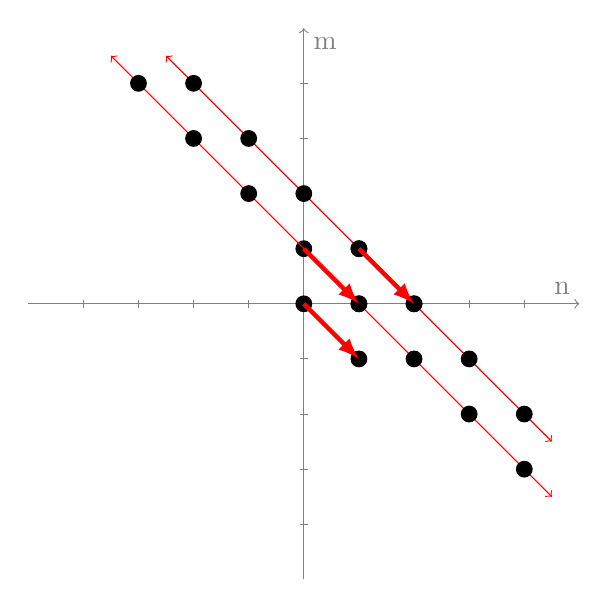
\begin{tikzpicture}[scale=.7]
\draw[thin, gray, ->] (0,-5) -- (0,5) node[anchor=north west] {m};
\draw[thin, gray, ->] (-5,0) -- (5,0) node[anchor=south east] {n};
\foreach \x in {-4,-3,-2,-1,1,2,3,4}
\draw[thin, gray] (\x,2pt) -- (\x,-2pt);
\foreach \y in {-4,-3,-2,-1,1,2,3,4}
\draw[thin, gray] (2pt,\y) -- (-2pt,\y);

\node[draw,circle,inner sep=2pt,fill] at (0,0) {};
\node[draw,circle,inner sep=2pt,fill] at (1,0) {};
\node[draw,circle,inner sep=2pt,fill] at (0,1) {};
\node[draw,circle,inner sep=2pt,fill] at (1,1) {};
\node[draw,circle,inner sep=2pt,fill] at (2,0) {};
\node[draw,circle,inner sep=2pt,fill] at (1,-1) {};

\draw [thin, red,-latex, <->] (-3.5,4.5) -- (4.5, -3.5) {};
\draw [thin, red,-latex, <->] (-2.5,4.5) -- (4.5, -2.5) {};

\foreach \x in {-3,-2,-1,1,2,3,4}
\node[draw,circle,inner sep=2pt,fill] at (\x,1 - \x) {};
\foreach \x in {-2,-1,0,1,2,3,4}
\node[draw,circle,inner sep=2pt,fill] at (\x,2 - \x) {};

\draw [ultra thick,-latex,red] (0,0) -- (1,-1) node [below] {$\zz$};
\draw [ultra thick,-latex,red] (0,1) -- (1,0) {};
\draw [ultra thick,-latex,red] (1,1) -- (2,0) {};
\end{tikzpicture}
\end{center}

Then for any $n \neq 0$, we may apply Lemma \ref{lem:generateline} to the triple
\[
    \xx = (n, 1-n), \quad \yy = (n, 2-n), \quad \zz = (0,1) 
\]
to generate the vertical line of points through $(n,0)$. 

\begin{center}
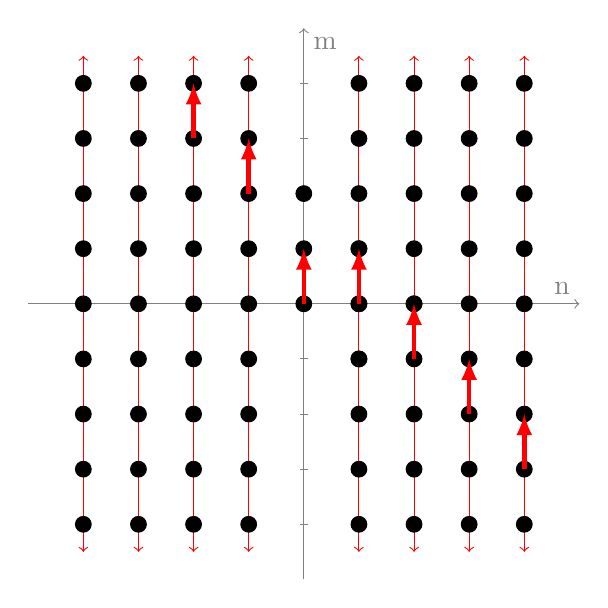
\begin{tikzpicture}[scale=.7]
\draw[thin, gray, ->] (0,-5) -- (0,5) node[anchor=north west] {m};
\draw[thin, gray, ->] (-5,0) -- (5,0) node[anchor=south east] {n};
\foreach \x in {-4,-3,-2,-1,1,2,3,4}
\draw[thin, gray] (\x,2pt) -- (\x,-2pt);
\foreach \y in {-4,-3,-2,-1,1,2,3,4}
\draw[thin, gray] (2pt,\y) -- (-2pt,\y);

\node[draw,circle,inner sep=2pt,fill] at (0,0) {};
\node[draw,circle,inner sep=2pt,fill] at (1,0) {};
\node[draw,circle,inner sep=2pt,fill] at (0,1) {};
\node[draw,circle,inner sep=2pt,fill] at (1,1) {};
\node[draw,circle,inner sep=2pt,fill] at (2,0) {};
\node[draw,circle,inner sep=2pt,fill] at (1,-1) {};

\draw [ultra thick,-latex,red] (0,0) -- (0,1) node [below left] {$\zz$};

\node[draw,circle,inner sep=2pt,fill] at (0,2) {};

\foreach \x in {-4,-3,-2,-1,1,2,3,4}
\draw [thin, red,-latex, <->] (\x, -4.5) -- (\x, 4.5) {};

\foreach \x in {-4,-3,-2,-1,1,2,3,4}
\foreach \y in {-4,-3,-2,-1,0,1,2,3,4}
\node[draw,circle,inner sep=2pt,fill] at (\x,\y) {};

\foreach \x in {-2,-1,1,2,3,4}
\draw [ultra thick,-latex,red] (\x,-\x + 1) -- (\x,-\x+2) {};

\end{tikzpicture}
\end{center}

Finally, any $\widetilde{P}_{0,m}$ for $m \neq 0$ can be expressed as
\[
    \widetilde{P}_{0,m} = \{ m \}^{-1} \Big( [\widetilde{P}_{1,m}, \widetilde{P}_{-1,0}] + \{ m \} \widetilde{P}_{2,m} \Big)
\]
which generates the last of what is left of the $\widetilde{P}_{n,m}$. This completes the proof.
\end{proof}

\begin{remark}
The proof above provides an algorithm for expressing any $\widetilde{P}_{n,m}$ in terms of the five generators. Of course, this expression is complicated, but it is not surprising since the generating set is so small.
\end{remark}






\subsection{Recalling Some Formulas From the Literature}

Let $\Lambda = (\Lambda_1, \dots, \Lambda_n)$ be a sequence of Young diagrams such that $|\Lambda_1|=1$, $|\Lambda_{i+1}| = |\Lambda_{i}| \pm 1$, and $\Lambda_n=\lambda$. 
We will call such a sequence an \textit{up-down tableau} of length $n$ and shape $\lambda(\Lambda) := \Lambda_n$. 
If $\Lambda = (\Lambda_1, \dots, \Lambda_{n-1}, \Lambda_n)$, then define $\Lambda' = (\Lambda_1, \dots, \Lambda_{n-1})$. 
In particular, $|\lambda(\Lambda)| = |\lambda(\Lambda')| \pm 1$. Following \cite{BB01}, recursively define morphisms $\fa_\Lambda$ and $\fb_\Lambda$ by:
\begin{align*}
    \fa_1 &:= \id_1 =: \fb_1 
\end{align*}
and if $|\Lambda_n| = |\Lambda_{n-1}| + 1$, then 
\begin{align*}
    \fa_\Lambda &:= (\fa_{\Lambda'} \otimes 1_1) \tilde{y}_{\Lambda(\Lambda)} \\
    \fb_\Lambda &:= \tilde{y}_{\lambda(\Lambda)} (\fb_{\Lambda'} \otimes 1_1)
\end{align*}
and if $|\Lambda_n| = |\Lambda_{n-1}| - 1$, then
\begin{align*}
    \fa_\Lambda &:= \frac{ \langle \Lambda_n \rangle}{ \langle \Lambda_{n-1} \rangle} (\fa_{\Lambda'} \otimes 1_1) (\tilde{y}_{\lambda(\Lambda)} \otimes \cap) \\
    \fb_\Lambda &:= (\tilde{y}_{\lambda(\Lambda)} \otimes \cup) (\fb_{\Lambda'} \otimes 1_1)
\end{align*}
where the morphisms $\cup \in \Hom_{\sfd(I^2)} \big( \varnothing, [2] \big)$ and $\cap \in \Hom_{\sfd(I^2)} \big( [2], \varnothing \big)$ are the obvious cup and cap morphisms, $\otimes$ is the monoidal product of $\sfd(I^2)$ induced by some standard embedding $I^2 \sqcup I^2 \to I^2$, and $\langle \lambda \rangle$ for a partition $\lambda$ is the quantum trace of a certain path idempotent in $BMW_n$ (see \cite{BB01} for details). 

\begin{theorem}[\cite{BB01}, Section 5] \label{thm:bmwbasis}
Let $d_\lambda^{(n)}$ be the number of up-down tableaux of length $n$ and shape $\lambda$. 
Let $\mathcal{M}_{d_\lambda}$ denote the $d_\lambda^{(n)} \times d_\lambda^{(n)}$ matrix algebra. 
Also, let
\[
    q_\Lambda := \alpha_\Lambda \beta_\Lambda, \qquad \qquad z_\lambda^{(n)}:= \sum_{\lambda(\Lambda)=\lambda} q_\Lambda
\]

\begin{enumerate} 
\item There is an algebra isomorphism
\[
    \rho: \underset{|\lambda| = n, n-2, \dots}{\bigoplus} \mathcal{M}_{d_{\lambda}^{(n)}} \overset{\sim}{\longrightarrow} BMW_n
\]
such that the image of a standard basis element is $\rho( e_{\Lambda,\Xi}^\lambda) = \alpha_\Lambda \beta_\Xi$ where $\lambda(\Lambda) = \lambda = \lambda(\Xi)$.
It follows that the $z_\lambda^{(n)}$ are central idempotents of $BMW_n$. \\
\item (Branching formula)
\[
    q_\Lambda \otimes 1_1 = \sum_{\Xi'=\Lambda} q_\Xi
\] 
for all up-down tableaux $\Lambda$, and
\[
\tilde{y}_\lambda \otimes \id_1 = \sum_{\substack{\lambda \subset \mu \\ \mu = \lambda + \square}} (\tilde{y}_\lambda \otimes \id_1) \tilde{y}_\mu (\tilde{y}_\lambda \otimes \id_1) + \sum_{\substack{\nu \subset \lambda \\ \lambda = \nu + \square}} \frac{\langle \nu \rangle}{\langle \lambda \rangle} (\tilde{y}_\lambda \otimes \id_1) (\tilde{y}_\nu \otimes c_1) (\tilde{y}_\lambda \otimes \id_1) 
\]
\item (Braiding coefficient)
\[
\tilde{y}_\mu (\tilde{y}_\lambda \otimes \id_1) \sigma_{n-1} \cdot \sigma_1 \sigma_1 \cdot \sigma_{n-1} \tilde{y}_\mu = s^{2\cn(\square)}\tilde{y}_\mu
\]
where the Young diagram of $\lambda$ is obtained by removing the cell $\square$ from the Young diagram of $\mu$.  
\item 
\[
    \fb_\Lambda \fa_\Lambda = \tilde{y}_{\lambda(\Lambda)}
\]
for all up-down tableaux $\Lambda$.
\end{enumerate}
\end{theorem}

\begin{remark} \label{rmk:qclosure}
Recall our notation $\widetilde{Q}_\lambda := \cl(\tilde{y}_\lambda)$. Then Theorem \ref{thm:bmwbasis} implies
\[
    \cl(q_\Lambda) = \cl(\fa_\Lambda \fb_\Lambda) = \cl(\fb_\Lambda \fa_\Lambda) = \cl(\tilde{y}_{\lambda(\Lambda)}) = \widetilde{Q}_{\lambda(\Lambda)},
\]
so therefore $\cl(z_\lambda^{(n)})$ is a positive integer multiple of $\widetilde{Q}_{\lambda(\Lambda)}$.
\end{remark}

Let's formally restate a theorem which was mentioned in Section \ref{sub:annulus}.

\begin{theorem}[\cite{LZ02}, Corollary 2, Proposition 2.1]\label{thm:ann_basis} 
$\,$
\begin{enumerate}
    \item The elements $\widetilde{Q}_\lambda$ form a basis of the skein module of a solid torus $\cd(I^2 \times S^1)$, where $\lambda$ ranges over all Young diagrams. 
    \item Let $\phi: \cc \to \cc$ be the meridian map so that $\phi(x)$ is a simple loop wrapped around $x$. Then
    \[
        \phi \big( \widetilde{Q}_\lambda \big) = c_\lambda \widetilde{Q}_\lambda
    \]
    where 
        \[c_\lambda = \delta_\cd + (s - s^{-1}) \Bigg( v^{-1}\sum_{x \in \lambda} s^{2\cn(x)} - v\sum_{x \in \lambda} s^{-2\cn(x)} \Bigg)
    \]
\end{enumerate}
\end{theorem}

This is the basis we will choose to act by $\cd(T^2)$ on in Section \ref{sec:action}. 


\subsection{Showing How Generators Act} \label{sec:action}

We will fix the convention that $\widetilde{P}_{1,0}$ acts as a meridian link and $\widetilde{P}_{0,1}$ acts as a longitude link. This next proposition shows how each element of the generating set of Proposition \ref{prop:generators} act.

\begin{proposition} \label{prop:generatoractions}
In the basis $\{ \widetilde{Q}_\lambda \}_\lambda$ of $\cd(I^2 \times S^1)$, the action of $\cd(T^2)$ is determined by the equations below.
\begin{align}
    \widetilde{P}_{1,0} \cdot \widetilde{Q}_\lambda &= \Bigg(\langle \widetilde{P}_1 \rangle + \{1\} \Big( v^{-1}\sum_{\square\in\lambda} s^{2\cn(\square)} - v \sum_{\square\in\lambda} s^{-2\cn(\square)} \Big) \Bigg) \widetilde{Q}_\lambda \label{eq:1,0}\\
    \widetilde{P}_{2,0} \cdot \widetilde{Q}_\lambda &= \Bigg(\langle \widetilde{P}_2 \rangle + \{2\} \Big( v^{-2}\sum_{\square\in\lambda} s^{4\cn(\square)} - v^2 \sum_{\square\in\lambda} s^{-4\cn(\square)} \Big) \Bigg) \widetilde{Q}_\lambda \label{eq:2,0}\\
    \widetilde{P}_{0,1} \cdot \widetilde{Q}_\lambda &= \sum_{\substack{\lambda \subset \mu \\ \mu = \lambda + \square}} \widetilde{Q}_\mu + \sum_{\substack{\nu \subset \lambda \\ \lambda = \nu + \square}} \widetilde{Q}_\nu \label{eq:0,1}\\
    \widetilde{P}_{1,1} \cdot \widetilde{Q}_\lambda &= v^{-1} \sum_{\substack{\lambda \subset \mu \\ \mu = \lambda + \square}} s^{2\cn(\square)} \widetilde{Q}_\mu + v \sum_{\substack{\nu \subset \lambda \\ \lambda = \nu + \square}} s^{-2\cn(\square)} \widetilde{Q}_\nu \label{eq:1,1}
\end{align}
\end{proposition}
\begin{proof}
The equation \eqref{eq:1,0} follows by considering the annular closure of the branching formula of Theorem \ref{thm:bmwbasis}, together with Remark \ref{rmk:qclosure}. 
Also, \eqref{eq:0,1} is precisely the result of the meridian map eigenvalue computation of Theorem \ref{thm:ann_basis}. Equation \eqref{eq:2,0} follows from Proposition \ref{prop:zlgeneralization} for $k=2$. All that's left to show is equation \eqref{eq:1,1}. To do this, we will apply the branching rule and braiding coefficient identities of Theorem \ref{thm:bmwbasis}. We will work with rectangular diagrams with the top edge identified with the bottom edge, creating annular diagrams. First, apply a framing relation and the branching rule
\begin{align*}
\pic{B11cdotQlambda.eps} &= v^{-1} \pic{B11cdotQlambdaframe.eps} \\
&= v^{-1} \sum_{\substack{\lambda \subset \mu \\ \mu = \lambda + \square}} \pic{B11cdotQlambdaframebrancha1.eps} + v^{-1} \sum_{\substack{\nu \subset \lambda \\ \lambda = \nu + \square}} \frac{\langle \nu \rangle}{\langle \lambda \rangle} \pic{B11cdotQlambdaframebranchb1.eps}
\end{align*}
where the first sum is over the set of partitions $\mu$ whose Young diagram is obtained by adding a single cell $\square$ to $\lambda$, and similarly for the second sum. Next, we can use the idempotent property to dubplicate and absorb idempotents. The right-hand side of the above equation becomes
\[
v^{-1} \sum_{\substack{\lambda \subset \mu \\ \mu = \lambda + \square}} \pic{B11cdotQlambdaframebrancha2.eps} + v^{-1} \sum_{\substack{\nu \subset \lambda \\ \lambda = \nu + \square}} \frac{\langle \nu \rangle}{\langle \lambda \rangle} \pic{B11cdotQlambdaframebranchb2.eps}.
\]
By the braiding coefficient formula, the diagram in the first sum is equal to $s^{2\cn(\square)} \widetilde{Q}_\mu$. The diagram in the second sum is calculated during the proof of Proposition 6.1 in \cite{BB01} to be $v^2 s^{-2\cn(\square)} \langle \lambda \rangle / \langle \nu \rangle \widetilde{Q}_\nu$. This completes the proof. 
\end{proof}










